% =====================================
% 【南京理工大学】Beamer 主题模板（Minimalist NJUST Beamer）
% 版式移植自 minimalist-pku-beamer-2026：
%   极简固定高度顶栏 + 右上角校徽 + 衬线排版 + 分节目录页 + 三线表
% 主题色：南理工紫 #990099（VI 标准色 C54 M96 Y0 K0 / Pantone 248 / RGB 153,0,153）
% 编译方式：XeLaTeX（latexmk -xelatex NJUST-slides.tex）
% 初版（ucas 风格）维护者：Shuai Qian (Andrew)，本版为其极简重制
% =====================================

% 画幅切换：aspectratio=43（4:3）↔ aspectratio=169（16:9，当前）
\documentclass[10pt,aspectratio=169,hyperref={colorlinks,citecolor=njust_blue,urlcolor=njust_blue,linkcolor=}]{beamer}
\usepackage{NJUST}
\usefonttheme{serif}

% 中文支持：需用 XeLaTeX 编译（latexmk -xelatex NJUST-slides.tex）
% 中文衬线宋体：macOS 用 Songti SC；Windows 用 SimSun（黑体代粗体）；
% 其他环境（Linux/Overleaf 等）自动回退到 TeX Live 自带的 FandolSong
% （按文件名经 kpathsea 加载，不依赖系统字体）
\usepackage[fontset=none, scheme=plain]{ctex}
\IfFontExistsTF{Songti SC}{%
  \setCJKmainfont{Songti SC}[AutoFakeSlant=0.2]%
  \setCJKsansfont{Songti SC}[AutoFakeSlant=0.2]%
  \setCJKmonofont{Songti SC}%
}{%
  \IfFontExistsTF{SimSun}{%
    \setCJKmainfont{SimSun}[BoldFont=SimHei,AutoFakeSlant=0.2,BoldItalicFont=SimHei,BoldItalicFeatures={FakeSlant=0.2}]%
    \setCJKsansfont{SimSun}[BoldFont=SimHei,AutoFakeSlant=0.2,BoldItalicFont=SimHei,BoldItalicFeatures={FakeSlant=0.2}]%
    \setCJKmonofont{FangSong}%
  }{%
    \setCJKmainfont{FandolSong-Regular}[Extension=.otf,BoldFont=FandolSong-Bold,AutoFakeSlant=0.2]%
    \setCJKsansfont{FandolSong-Regular}[Extension=.otf,BoldFont=FandolSong-Bold,AutoFakeSlant=0.2]%
    \setCJKmonofont{FandolFang-Regular}[Extension=.otf,BoldFont=FandolFang-Regular]%
  }%
}
\usepackage{hyperref}
\setmainfont{XCharter} % 衬线拉丁字体（TeX Live 自带）
% 等宽字体：优先 Maple Mono NF（静态字族，真实粗/斜体），其次可变版，未安装则回退默认
\IfFontExistsTF{Maple Mono NF}{%
  \setmonofont{Maple Mono NF}[Scale=MatchLowercase,Ligatures=TeX]%
}{%
  \IfFontExistsTF{Maple Mono}{%
    \setmonofont{Maple Mono}[Scale=MatchLowercase,Ligatures=TeX]%
  }{}%
}
% other packages
\usepackage{latexsym,amsmath,xcolor,multicol,booktabs,calligra}
\usepackage{amssymb}
\usepackage{graphicx}
\usepackage{tikz}
\usepackage{bm}
\usepackage{natbib}
\usepackage{wrapfig}
\usepackage{amsfonts}
\usepackage{ragged2e}
\usepackage{parskip}

\apptocmd{\frame}{}{\justifying}{} % Allow optional arguments after frame.

% 引用整体着色为 njust_blue（与 definition block 标题蓝一致）：
% natbib 的 \citep/\citet 括号不在 hyperref 链接内，仅靠 citecolor 只能染色链接部分，
% 此处将整个引用（含括号）包进颜色组。
\makeatletter
\NewCommandCopy{\njust@citep@orig}{\citep}
\NewCommandCopy{\njust@citet@orig}{\citet}
\RenewDocumentCommand{\citep}{o o m}{%
  \begingroup\color{njust_blue}%
  \IfNoValueTF{#1}{\njust@citep@orig{#3}}%
    {\IfNoValueTF{#2}{\njust@citep@orig[][#1]{#3}}%
      {\njust@citep@orig[#1][#2]{#3}}}%
  \endgroup}
\RenewDocumentCommand{\citet}{o o m}{%
  \begingroup\color{njust_blue}%
  \IfNoValueTF{#1}{\njust@citet@orig{#3}}%
    {\IfNoValueTF{#2}{\njust@citet@orig[][#1]{#3}}%
      {\njust@citet@orig[#1][#2]{#3}}}%
  \endgroup}
\makeatother

\newcommand{\theHalgorithm}{\arabic{algorithm}}
\theoremstyle{plain}
\newtheorem{axiom}{Axiom}
\newtheorem{claim}[axiom]{Claim}
\newtheorem{assumption}{Assumption}
\newtheorem{remark}{Remark}


% 修改为你的标题页信息
\author[张三]{张三\\{\small\href{mailto:zhangsan@njust.edu.cn}{\texttt{zhangsan@njust.edu.cn}}}}
\title[Minimalist NJUST Beamer]{南京理工大学 Beamer 主题模板}
\subtitle{Minimalist NJUST Beamer · 南理工紫主题}
\institute{XX 学院，南京理工大学}
\date{2026/09/23}

% 右上角校徽（与标题条同高、严格对齐）由 NJUST.sty 中的 frametitle 模板绘制
\def\cmd#1{\texttt{\color{red}\footnotesize $\backslash$#1}}
\def\env#1{\texttt{\color{blue}\footnotesize #1}}
\definecolor{deepblue}{rgb}{0,0,0.5}
\definecolor{deepred}{rgb}{0.6,0,0}
\definecolor{deepgreen}{rgb}{0,0.5,0}
\definecolor{halfgray}{gray}{0.55}

\begin{document}
{
\setbeamertemplate{logo}{}
\begin{frame}
    \titlepage
    \begin{figure}[htpb]
        \begin{center}
            
\includegraphics[width=0.3\linewidth]{logo/NJUST.png}
        \end{center}
    \end{figure}
\end{frame}
}

\section{PX4 简介}

\begin{frame}{开源飞行控制软件——PX4}
\begin{block}{官网介绍}
PX4 is an open source \textbf{flight control software} for drones and other unmanned vehicles. The project provides a flexible set of tools for drone developers to share technologies to create tailored solutions for drone applications. PX4 provides a standard to deliver drone \textbf{hardware} support and \textbf{software} stack, allowing an ecosystem to build and maintain hardware and software in a scalable way \citep{px4website}.
\end{block}

\begin{itemize}
    \item 官网：\url{https://px4.io/}
    \item 代码管理：\url{https://github.com/PX4/PX4-Autopilot}
    \item 开发者手册：\url{https://docs.px4.io/}
\end{itemize}
\end{frame}

\begin{frame}{PX4 固件版本}
	\begin{itemize}
		\item 最新发布稳定版本\footnote{\url{https://github.com/PX4/PX4-Autopilot/releases}}：v1.11.2
		\item 使用版本：v1.10.0
	\end{itemize}
	\begin{figure}
		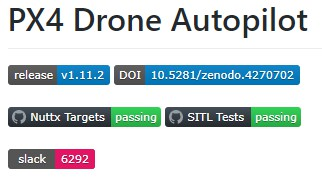
\includegraphics[width=0.3\linewidth]{image/release.jpg}
		\caption{PX4 软件版本}
	\end{figure}
	不同版本的固件会修改 bug、增加新功能，例如：v1.10.0 将多旋翼 IMU 数据更新速率提高到 1\,kHz，v1.10.1 为了减小 CPU 负载又将其降为 400\,Hz。
\end{frame}

\begin{frame}{PX4 系统架构概述}
	\citet{meier2015px4} 将 PX4 的实现划分为两个主要部分：
	\begin{itemize}
		\item \textbf{飞行控制栈}（flight stack）：主要包括状态估计和飞行控制系统；
		\item \textbf{中间件}：通用的机器人应用层，负责内部/外部通讯和硬件整合。
	\end{itemize}
	所有 PX4 支持的机型（含无人船、无人车、无人水下航行器等）共用同一代码库。
	\begin{figure}
		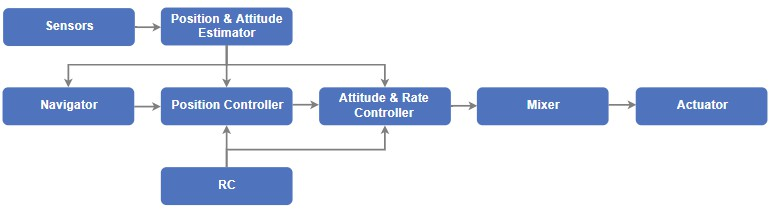
\includegraphics[width=0.55\linewidth]{image/stack.jpg}
		\caption{PX4 飞行控制栈\footnote{\url{https://docs.px4.io/main/zh/concept/architecture.html}}}
	\end{figure}
\end{frame}

\section{主要内容}

\begin{frame}{文本区块}
  将文本放入区块内

  \begin{block}{普通区块}
    这是普通色块（辅助蓝）
  \end{block}

  \begin{exampleblock}{示例区块}
    这是示例色块（浅紫金），\red{红色}、\green{绿色}为便捷文本颜色命令
  \end{exampleblock}

  \begin{alertblock}{强调区块}
    强调色为紫金（\texttt{njust\_gold}），与定理类区块一致
  \end{alertblock}
\end{frame}

\begin{frame}{三线表}
    \begin{table}
        \caption{PX4 固件版本对照}
        \label{tab:px4}
        \setlength{\parskip}{0pt}% caption 与表头之间不插入段间距
        \footnotesize
        \setlength{\tabcolsep}{3pt}
        \begin{tabular}{p{50pt}p{70pt}p{190pt}}
        \toprule
        {\bfseries 版本}&
        {\bfseries 发布状态}&
        {\bfseries 主要变化} \\
        \midrule
        v1.10.0&
        使用版本&
        多旋翼 IMU 数据更新速率 1\,kHz \\
        v1.10.1&
        过渡版本&
        为了减小 CPU 的负载，将该速率降为 400\,Hz \\
        v1.11.2&
        最新稳定版&
        修复若干缺陷、增加新的功能（演示数据）\citep{px4docs} \\
        \bottomrule
        \multicolumn{3}{p{310pt}}{三线表由 \texttt{booktabs} 绘制：头尾粗线 1.2\,pt，中间线 0.5\,pt；表头加粗（黑色）。}
        \end{tabular}
    \end{table}
\end{frame}

\begin{frame}{定理与证明}
\begin{theorem}[具体与连续]\label{thm:concrete}
  任何具体对象都可以分解为\textbf{连续}与\textbf{离散}两部分：
  \[
    \textbf{具体} = \textbf{连续} + \textbf{离散}.
  \]
\end{theorem}

\begin{proof}
  以函数为例：连续部分体现为积分，离散部分体现为级数求和，
  \begin{equation}\label{eq:alpha}
    \alpha = \beta + \gamma.
  \end{equation}
  这里还可以引用定理~\ref{thm:concrete}。
\end{proof}
\end{frame}

\begin{frame}{自定义字体大小}
  \begin{center}
    \begin{tabular}{ll}
      \Huge  $\backslash$Huge                & \Huge \structure{24.88 pt}     \\
      \huge  $\backslash$huge                & \huge \structure{20.74 pt}     \\
      \LARGE $\backslash$LARGE               & \LARGE \structure{17.28 pt}    \\
      \Large $\backslash$Large               & \Large \structure{14.4 pt}     \\
      \large $\backslash$large               & \large \structure{12 pt}       \\
      \normalsize $\backslash$normalsize     & \normalsize \structure{10 pt}  \\
      \small $\backslash$small               & \small \structure{9 pt}        \\
      \footnotesize $\backslash$footnotesize & \footnotesize \structure{8 pt} \\
      \scriptsize $\backslash$scriptsize     & \scriptsize \structure{7 pt}   \\
      \tiny $\backslash$tiny                 & \tiny \structure{5 pt}
    \end{tabular}
  \end{center}
\end{frame}

\section{总结}

\begin{frame}{总结}
\begin{itemize}
    \item 本模板版式：固定高度顶栏、右上角校徽墨迹对齐、分节目录页、编号定理环境
    \item 主题色为南理工紫 \texttt{\#990099}（VI 标准色 C54 M96 Y0 K0 / Pantone 248）
    \item 区块配色：辅助蓝（定义/普通区块）、紫金（定理/强调）、浅紫金（示例）
    \item 使用 XeLaTeX 一键编译：\texttt{latexmk -xelatex NJUST-slides.tex}
\end{itemize}
\end{frame}

\begin{frame}{参考文献}
    \renewcommand*{\bibfont}{\footnotesize}
    \bibliography{ref}
    \bibliographystyle{apalike}
\end{frame}

\begin{frame}
    \begin{center}
        {\Huge\calligra Thanks!}
    \end{center}
\end{frame}

\end{document}
